\documentclass[nooutcomes,noauthor,hints]{ximera}

\graphicspath{  
{./}
{./whoAreYou/}
{./drawingWithTheTurtle/}
{./bisectionMethod/}
{./circles/}
{./anglesAndRightTriangles/}
{./lawOfSines/}
{./lawOfCosines/}
{./plotter/}
{./staircases/}
{./pitch/}
{./qualityControl/}
{./symmetry/}
{./nGonBlock/}
}


%% page layout
\usepackage[cm,headings]{fullpage}
\raggedright
\setlength\headheight{13.6pt}


%% fonts
\usepackage{euler}

\usepackage{FiraMono}
\renewcommand\familydefault{\ttdefault} 
\usepackage[defaultmathsizes]{mathastext}
\usepackage[htt]{hyphenat}

\usepackage[T1]{fontenc}
\usepackage[scaled=1]{FiraSans}

%\usepackage{wedn}
\usepackage{pbsi} %% Answer font


\usepackage{cancel} %% strike through in pitch/pitch.tex


%% \usepackage{ulem} %% 
%% \renewcommand{\ULthickness}{2pt}% changes underline thickness

\tikzset{>=stealth}

\usepackage{adjustbox}

\setcounter{titlenumber}{-1}

%% journal style
\makeatletter
\newcommand\journalstyle{%
  \def\activitystyle{activity-chapter}
  \def\maketitle{%
    \addtocounter{titlenumber}{1}%
                {\flushleft\small\sffamily\bfseries\@pretitle\par\vspace{-1.5em}}%
                {\flushleft\LARGE\sffamily\bfseries\thetitlenumber\hspace{1em}\@title \par }%
                {\vskip .6em\noindent\textit\theabstract\setcounter{question}{0}\setcounter{sectiontitlenumber}{0}}%
                    \par\vspace{2em}
                    \phantomsection\addcontentsline{toc}{section}{\thetitlenumber\hspace{1em}\textbf{\@title}}%
                     }}
\makeatother



%% thm like environments
\let\question\relax
\let\endquestion\relax

\newtheoremstyle{QuestionStyle}{\topsep}{\topsep}%%% space between body and thm
		{}                      %%% Thm body font
		{}                              %%% Indent amount (empty = no indent)
		{\bfseries}            %%% Thm head font
		{)}                              %%% Punctuation after thm head
		{ }                           %%% Space after thm head
		{\thmnumber{#2}\thmnote{ \bfseries(#3)}}%%% Thm head spec
\theoremstyle{QuestionStyle}
\newtheorem{question}{}



\let\freeResponse\relax
\let\endfreeResponse\relax

%% \newtheoremstyle{ResponseStyle}{\topsep}{\topsep}%%% space between body and thm
%% 		{\wedn\bfseries}                      %%% Thm body font
%% 		{}                              %%% Indent amount (empty = no indent)
%% 		{\wedn\bfseries}            %%% Thm head font
%% 		{}                              %%% Punctuation after thm head
%% 		{3ex}                           %%% Space after thm head
%% 		{\underline{\underline{\thmname{#1}}}}%%% Thm head spec
%% \theoremstyle{ResponseStyle}

\usepackage[tikz]{mdframed}
\mdfdefinestyle{ResponseStyle}{leftmargin=1cm,linecolor=black,roundcorner=5pt,
, font=\bsifamily,}%font=\wedn\bfseries\upshape,}


\ifhandout
\NewEnviron{freeResponse}{}
\else
%\newtheorem{freeResponse}{Response:}
\newenvironment{freeResponse}{\begin{mdframed}[style=ResponseStyle]}{\end{mdframed}}
\fi



%% attempting to automate outcomes.

%% \newwrite\outcomefile
%%   \immediate\openout\outcomefile=\jobname.oc
%% \renewcommand{\outcome}[1]{\edef\theoutcomes{\theoutcomes #1~}%
%% \immediate\write\outcomefile{\unexpanded{\outcome}{#1}}}

%% \newcommand{\outcomelist}{\begin{itemize}\theoutcomes\end{itemize}}

%% \NewEnviron{listOutcomes}{\small\sffamily
%% After answering the following questions, students should be able to:
%% \begin{itemize}
%% \BODY
%% \end{itemize}
%% }
\usepackage[tikz]{mdframed}
\mdfdefinestyle{OutcomeStyle}{leftmargin=2cm,rightmargin=2cm,linecolor=black,roundcorner=5pt,
, font=\small\sffamily,}%font=\wedn\bfseries\upshape,}
\newenvironment{listOutcomes}{\begin{mdframed}[style=OutcomeStyle]After answering the following questions, students should be able to:\begin{itemize}}{\end{itemize}\end{mdframed}}



%% my commands

\newcommand{\snap}{{\bfseries\itshape\textsf{Snap!}}}
\newcommand{\flavor}{\link[\snap]{https://snap.berkeley.edu/}}
\newcommand{\mooculus}{\textsf{\textbf{MOOC}\textnormal{\textsf{ULUS}}}}


\usepackage{tkz-euclide}
\tikzstyle geometryDiagrams=[rounded corners=.5pt,ultra thick,color=black]
\colorlet{penColor}{black} % Color of a curve in a plot



\ifhandout\newcommand{\mynewpage}{\newpage}\else\newcommand{\mynewpage}{}\fi

\title{Formulas galore}

\author{Bart Snapp}

\begin{document}
\begin{abstract}
  Let's think about formulas.
\end{abstract}
\maketitle


\begin{listOutcomes}
\item Apply formulas to compute the surface areas and volumes of
  solids.
\item Acknowledge that even with a formula, difficult work still needs
  to be done.
\item Evaluate estimates as either too large or too small.
\end{listOutcomes}


Here are a bunch of formulas I found on the INTERNET at this site
\begin{center}
  \textit{https://sites.google.com/site/standardbasicengineering/home/useful-formula-for-finding-area-volume-of-solid-figures}
\end{center}
\begin{center}
  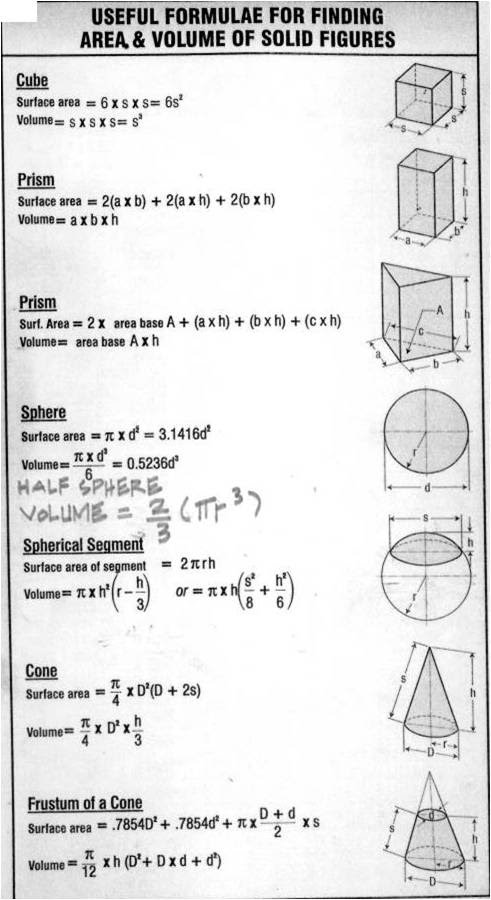
\includegraphics[width=.3\textwidth]{photoFormula1.jpg} \qquad 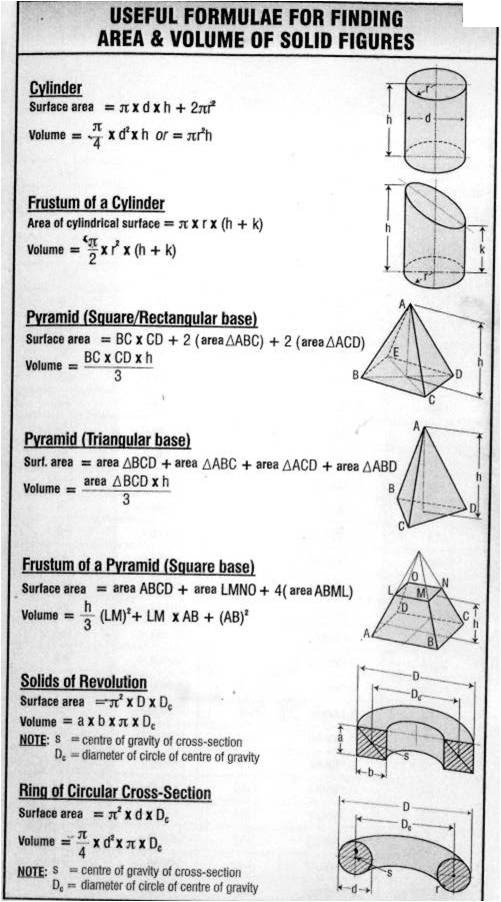
\includegraphics[width=.3\textwidth]{photoFormula2.jpg}
\end{center}

Below, let's think about some questions. 


\mynewpage




\begin{question}
  Consider the \link[\textit{Ericsson Globe}]{https://en.wikipedia.org/wiki/Ericsson_Globe}:
   \begin{center}
    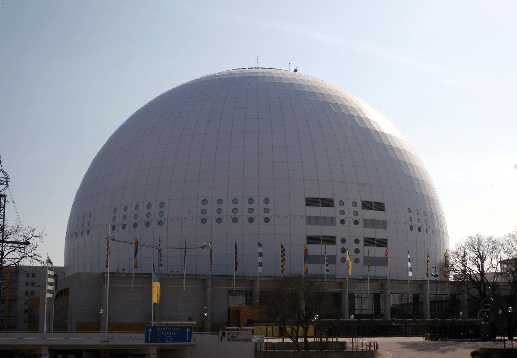
\includegraphics[width=.4\textwidth]{dome.png} %https://www.researchgate.net/figure/Example-of-a-hemispherical-dome-in-modern-civil-engineering-Stockholm-Globe-Arena-by_fig2_308655043
   \end{center}
   Assuming that this building has a diameter of $110$ meters and a
   height of $85$ meters.
   \begin{enumerate}
   \item \label{FG1:1} Use the formulas above to find the surface area
     and the volume of the \textit{Ericsson Globe}.
   \item Estimate the values above by finding the surface area and
     volume of:
     \begin{enumerate}
     \item A box with dimensions $100\times 100 \times 80$.
     \item A box with dimensions $100\times 80 \times 80$.
     \end{enumerate}
   Note: While these answers are NOT EQUAL to your answers from
   part \ref{FG1:1}, these answers \textbf{HAVE THE SAME NUMBER OF
     DIGITS} as your answers from part \ref{FG1:1}.
   \end{enumerate}
   \begin{freeResponse}
     \begin{enumerate}
     \item Using the formulas above I found:
       \[
       SA = 2\pi 55\cdot 85 \approx 29374 \text{ square meters}
       \]
       and
       \[
       V = \pi85^2 \left(55-\frac{85}{3}\right)\approx  605280 \text{ cubic meters}.
       \]
     \item We have two computations.
       \begin{enumerate}
       \item For a box that is  $100\times 100 \times 80$, I find
         \[
         SA = 2(100\cdot 100 + 100\cdot 80 + 100\cdot 80) = 52000 
         \]
         and
         \[
         V = 100\cdot 100\cdot 80 =  800000 
         \]
       \item For a box that is  $100\times 80 \times 80$, I find
         \[
         SA = 2(100\cdot 80 + 80\cdot 80 + 100\cdot 80) = 44800
         \]
         and
         \[
         V = 100\cdot 80\cdot 80 = 640000
         \] 
       \end{enumerate}
       Yup, these answers have the same number of digits as our answers from the first part.       
     \end{enumerate}
   \end{freeResponse}
\end{question}
\mynewpage




%%%%%%%%%%%%%%%%%%%%%%%%
%%%%%% COULD BE IT's OWN ACTIVITY
%%% UPPER AND LOWER BOUNDS

\begin{question}
  Consider the \link[\textit{Luxor Las Vegas}]{https://en.wikipedia.org/wiki/Luxor_Las_Vegas}:
  \begin{center}
    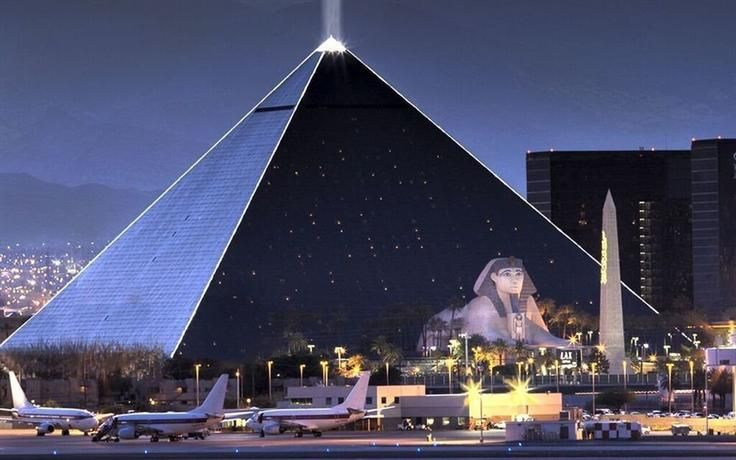
\includegraphics[width=.4\textwidth]{pyramid.jpg} 
  \end{center}
 Assuming that the (square) base of this building has a side length of
 $646$ feet and that the pyramid is $350$ feet tall,
  \begin{enumerate}
  \item Which is EASIER to compute:
    \begin{itemize}
    \item the surface area (NOT including the bottom!) OR
    \item the volume
    \end{itemize}
    of the \textit{Luxor Las Vegas}? EXPLAIN WHY one computation is
    HARDER, and compute the EASIER one.
  \item %% FOR THIS: ESTIMATE BY BASE AREA, ESTIMATE WITH 4 upright tri and place the correct value. 

    You ask six friends what the surface area of the top part of the
    \textit{Luxor Las Vegas} is. They give you six wrong answers, but
    you love them anyway, because they are your friends. Here are
    their answers:
    \begin{enumerate}
    \item $650$ square feet
    \item $6500$ square feet
    \item $65000$ square feet
    \item $650000$ square feet
    \item $6500000$ square feet
    \item $65000000$ square feet
    \end{enumerate}
    Which answer above is \textbf{closest} to the correct answer? EXPLAIN your reasoning.
  \end{enumerate}
  \begin{freeResponse}
    \begin{enumerate}
      \item The volume is MUCH EASIER to compute than the surface
        area. To compute the surface area, you have to compute the
        area of each face of the pyramid, this requires GEOMETRY.

        The volume is
        \[
        V = \frac{646\cdot 646\cdot 350}{3} \approx = 48686867 \text{ cubic feet}.
        \]
      \item Answer $(iv)$ is correct, here's how I know. The pyramid
        has a base, and four more sides. The BIGGEST the surface area could be is
        \[
        4\cdot 350\cdot 646 = 904400.
        \]
        On the other hand, the area of the SMALLEST the surface area could be is
        the area of the base, or
        \[
        646\cdot 646 = 417316.
        \]
        Note, $417316 < 650000 <  904400$.        
    \end{enumerate}
  \end{freeResponse}
\end{question}
\mynewpage



\begin{question}
  Formulas can be hard to use, sometimes a good guess is best.
  \begin{enumerate}
  \item Here is a roof that is pointed in the middle:
  \begin{center}
    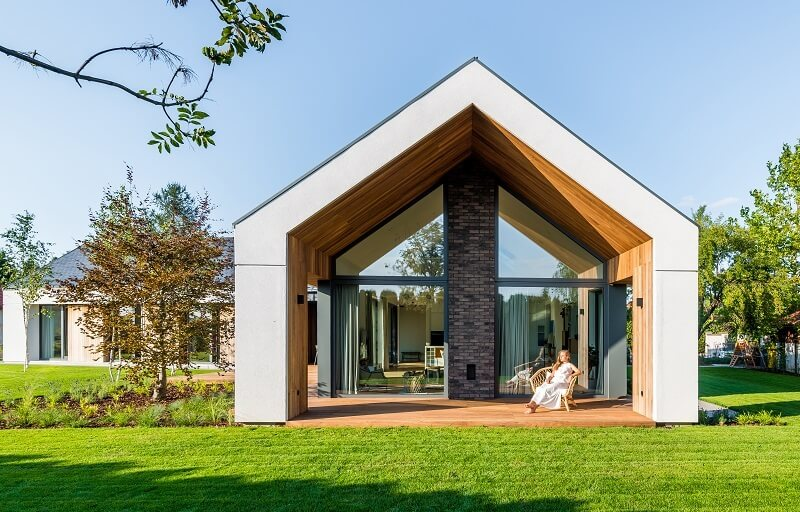
\includegraphics[width=.6\textwidth]{symRoof.jpg}
  \end{center}
  Below is a diagram of the roof as seen from the top:
  \begin{center}
    \begin{tikzpicture}[x=2cm,y=2cm]
      \draw[ultra thick] (0,0) rectangle (3,2.4);
      %\draw[dashed] (.5,.5) rectangle (4.3,2.5);
    \draw[ultra thick] (0,1.2) -- (3,1.2);
    \draw[decoration={brace,raise=.2cm},decorate,thin] (0,0)--(0,2.4);
    \draw[decoration={brace,raise=.2cm,mirror},decorate,thin] (0,0)--(3,0);
    \node at (-.4,1.2) {$24'$};
    \node at (1.5,-.44) {$30'$};
    \node[above] at (1.5,1.2) {main ridge};
    \end{tikzpicture}
  \end{center}
  You ask four friends what the surface area of the root is. They give
  you for wrong answers. Here are their answers:
    \begin{enumerate}
    \item $9$ square feet
    \item $90$ square feet
    \item $900$ square feet
    \item $9000$ square feet
    \end{enumerate}
    Which answer above is \textbf{closest} to the correct answer? EXPLAIN your reasoning.
  \item Here is a roof with an asymmetric roof:
  \begin{center}
    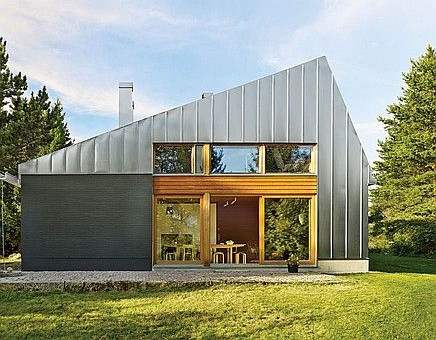
\includegraphics[width=.6\textwidth]{skewRoof.jpg}
  \end{center}
  Below is a diagram of the roof as seen from the top:
\begin{center}
  \begin{tikzpicture}[x=1.5cm,y=1.5cm]
    \draw[ultra thick] (0,0) rectangle (5,3.6);
    %\draw[dashed] (.3,.3) rectangle (4.5,2.1);
    \draw[ultra thick] (0,3) -- (5,3);
    \draw[decoration={brace,raise=.2cm},decorate,thin] (0,0)--(0,3);
    \draw[decoration={brace,raise=.2cm,mirror},decorate,thin] (5,3.1)--(5,3.6);
    \draw[decoration={brace,raise=.2cm,mirror},decorate,thin] (0,0)--(5,0);
    \node at (-.5,1.5) {$30'$};
    \node at (5.4,3.3) {$6'$};
    \node at (2.5,-.44) {$50'$};
    \node[below] at (2.5,3) {main ridge};
  \end{tikzpicture}
\end{center}
  You ask four friends what the surface area of the root is. They give
  you for wrong answers. Here are their answers:
    \begin{enumerate}
    \item $20$ square feet
    \item $200$ square feet
    \item $2000$ square feet
    \item $20000$ square feet
    \end{enumerate}
    Which answer above is \textbf{closest} to the correct answer? EXPLAIN your reasoning.
  \end{enumerate}
  \begin{freeResponse}
    \begin{enumerate}
    \item Answer $(iii)$ is correct. The SMALLEST that the area of the
      roof could be is
      \[
      24\cdot 30 = 720.
      \]
      It is clear that the length of a side is around $12$ feet (half the width), so
      the LARGEST the are of the roof could be is
      \[
      \underbrace{720}_{\text{area of base}} + 2\cdot 12\cdot 30 = 1440.
      \]
      Note, $720 < 900 < 1440$.
    \item Answer $(iv)$ is correct.  The SMALLEST that the area of the
      roof could be is
      \[
      36\cdot 50 = 1800.
      \]
      The average of each side of the roof is a little greater than
      have of the width, so the LARGEST the are of the roof could be
      is
      \[
      \underbrace{1800}_{\text{area of base}} + 2\cdot 18\cdot 50 = 3600.
      \]
      Note, $1800 < 2000 < 3600$.
    \end{enumerate}
  \end{freeResponse}
\end{question}
\mynewpage


\end{document}
